\documentclass[11pt]{article}
\usepackage{amsmath}
\usepackage{algpseudocode,algorithm}
\usepackage{subfigure}
\usepackage{graphicx}
\usepackage{psfrag,color}
\usepackage{fullpage}
\usepackage{epsfig}
\usepackage{amssymb}
\usepackage{titlesec}
\usepackage{minted}

\titleformat{\section}
  {\normalfont\large\bfseries}   
  {}
  {0pt}
  {}

\titleformat{\subsection}
  {\normalfont\bfseries}   
  {}
  {0pt}
  {}

\setlength{\textwidth}{6.5in}
\setlength{\oddsidemargin}{0.0in}
\setlength{\textheight}{9.0in}
\setlength{\parindent}{0in}

\renewcommand\arraystretch{2.4}

\renewcommand{\baselinestretch}{1.2}
\newcommand{\problem}[1]{ \medskip \pp $\underline{\rm Problem\ #1}$\\ }

\pagestyle{empty}

\def\pp{\par\noindent}

\begin{document}

\centerline{\{\bf Amy Qi, xq2224\}}
\centerline{\bf Homework 1 Solutions}
\centerline{\bf CS4771 --- Fall 2023}

\bigskip 
\bigskip

\section{Problem 1}
\subsection{(a)}
The first image $a = (0,0,...,0)$. The second image $b = (255,255,...,255)$. \\
Euclidean distance between these two images is
\begin{equation}
    \begin{split}
        ||a-b|| &= \sqrt{(a_1-b_1)^2 + (a_2-b_2)^2 +\ldots+(a_{784}-b_{784})^2} \\
        &= \sqrt{(0-255)^2 + (0-255)^2 +\ldots+(0-255)^2} \\
        &= 7140
    \end{split}
\end{equation}

% \bigskip
\subsection{(b)}
The average value of $||x-NN(x;S_{MNIST}||$ is 1254922.3729. \\
Its square root is 1120.2331779143126. \\
Code attached below.
\begin{minted}[breaklines]{python}
# Imports shared by all code snippets in this assignment
import pickle
import matplotlib.pyplot as plt
import numpy as np
import math
import scipy.stats as stats # this is just for plotting

def learn(train_x, train_y):
    return (train_x.astype(float), train_y)
model = learn(mnist['data'], mnist['labels'])
    
def find_avg(params, test_x):
    x, y = params
    return np.average(np.min(((np.sum(x**2, axis=1) - 2*test_x.dot(x.T)).T + np.sum(test_x**2, axis=1)).T, axis=1))
avg_dist = find_avg(model, mnist['testdata'].astype(float))
avg_dist_sqrt = math.sqrt(avg_dist)
\end{minted}

% \bigskip
\subsection{(c)}
Test error rate of the NN classifier with these "noisy" images is 0.0382. Code attached below. Imports omitted.
\begin{minted}[breaklines]{python}
# adding random bits to training dataset
train_x = mnist['data'].astype(float) # shape (60000,784)
rng = np.random.default_rng()
train_x_noise = rng.integers(255, size=(60000,280))
trainx = np.hstack((train_x,train_x_noise))

# adding random bits to test dataset
test_x = mnist['testdata'].astype(float) # shape (10000,784)
rng = np.random.default_rng()
test_x_noise = rng.integers(255, size=(10000,280))
testx = np.hstack((test_x,test_x_noise))

# run NN algorithm
result2 = predict((trainx,mnist['labels']), testx)

# calculate test error rate
error_count = 0
for i in range(len(result2)):
    if(result2[i] != mnist['testlabels'][i]):
        error_count+=1
test_error_rate = error_count/len(mnist['testdata'])
\end{minted}

% \bigskip
\subsection{(d)}
When $k=n$ where $n$ is the number of training examples, kNN actually returns the most frequent number in the dataset as the predicated class label for every single input. The property is thus the mode of the class labels in the training dataset. In this dataset it's 1, and the error rate of this dataset is $0.8876333333333334$.\\
% For example, if the entire training set is made up of numbers classified as $1$, then the training error rate will be $0$ because all values will be correctly predicted. However, for a dataset with greater variance, such as the MNIST dataset with $var=6172.850482291254$, the training error rate is much greater. The error rate of this dataset is $0.8876333333333334$. \\
Code attached below. Imports omitted.
\begin{minted}[breaklines]{python}
# function for kNN when k=n
def knn_predict(params, test_x):
    x, y = params
    unique, counts = np.unique(y, return_counts=True)
    print(dict(zip(unique, counts))) # number of occurences of each class value

knn_predict(model, mnist['data'].astype(float))
# prints {0: 5923, 1: 6742, 2: 5958, 3: 6131, 4: 5842, 5: 5421, 6: 5918, 7: 6265, 8: 5851, 9: 5949}
# the mode in this dataset is 1

# calculate the error rate
error_count = 0
for i in range(len(mnist['data'])):
    if(mnist['labels'][i] != 1): # known from knn_predict that the mode is 1
        error_count+=1
print(error_count/len(mnist['data']))
\end{minted}

\pagebreak
\section{Problem 2}
To show that two functions are the same, we want to show regardless of the distance function we use in the classifier, the output class for the same input test vector will always be the same. This means that the pair of vectors that are the "closest" remain the "closest" even after we change the distance function, i.e., for test data $(X_i,Y_i)$, both $f_1$ and $f_2$ return the same training data $(X_j,Y_j)$ as it minimizes both functions.

\subsection{(a)}
These two functions are different. Here is a counterexample. \\
Suppose feature vector $\Vec{a}=(1,0)$ and feature vector $\Vec{b}=(\frac{1}{2},\frac{2}{3})$ are two vectors in the training dataset. Consider feature vector $\Vec{c}=(0,0)$ in the test dataset. Using distance function $D(x,z)=||x-z||_1$, $D(a,c)=|1-0|+|0-0|=1$, $D(b,c)=|\frac{1}{2}-0|+|\frac{2}{3}-0|=\frac{7}{6}$. Since $D(a,c)<D(b,c)$, the classification result is the label attached to $\Vec{a}$.\\
Now consider distance function $D(x,z)=||x-z||_4$. $D(a,c)=((1-0)^4+(0-0)^4)^{\frac{1}{4}}=1$, $D(b,c)=((\frac{1}{2}-0)^4+(\frac{2}{3}-0)^4)^{\frac{1}{4}}\approx0.71$. Since $D(a,c)>D(b,c)$, the classification result is the label attached to $\Vec{b}$.\\
Substituting the distance function results in different classification result, therefore the pair of functions are note equal.

\subsection{(b)}
These two functions are the same. \\
Suppose for any input vector $\Vec{a}=(x_1,x_2,\ldots,x_n)$, using $D(x,z)=||x-z||$, the vector that is the closest to $\Vec{a}$ is $\Vec{b}=(y_1,y_2,\ldots,y_n)$. We want to show that for the same input vector $\Vec{a}$, using $D(x,z)=||x-z||^2$, the vector that is the closest to $\Vec{a}$ is still $\Vec{b}$. \\
Consider the case when we use $D(x,z)=||x-z||$. This means that $\sqrt{(x_1-y_1)^2+\ldots+(x_n-y_n)^2}$ is the minimum for this pair of vectors. Now consider $D(x,z)=||x-z||^2$, which is essentially squaring that value, i.e., $(x_1-y_1)^2+\ldots+(x_n-y_n)^2$. It should still be the smallest value out of all pairs of $\Vec{a}$ and $\Vec{b_i}$ for all $i$s. Therefore the classification result does not change and the two functions are the same.

\subsection{(c)}
At most 1. \\
Since $||x-z||_1=1$, we know $|x_1-z_1|+|x_2-z_2|+\ldots+|x_n-z_n|=1$, which indicates that $0\leq|x_i-z_i|\leq1$ for all integer $1\leq i\leq n$. \\
Now consider $||x-z||_3=(|x_1-z_1|^3+|x_2-z_2|^3+\ldots+|x_n-z_n|^3)^{\frac{1}{3}}$, when each term $0\leq|x_i-z_i|\leq1$ gets cubed, its value gets even smaller, so the sum of all these terms will be less than $1$. When a number less than $1$ gets raised to the power of $\frac{1}{3}$, the value cannot be greater than $1$ since $f(x)=x^{\frac{1}{3}}$ monotonically increases for $x>0$ and $f(1)=1$. Therefore the value is at most 1.

\newpage
\section{Problem 3}
\subsection{(a)}
Use random variable $X$ to denote the number of heads out of four coin tosses. \\
Then the probability of exactly two or three tosses come up heads is 
\begin{equation}
    \begin{split}
        P(X=2 \lor X=3) &= P(X=2) + P(X=3) \\
        &= \binom{4}{2}(\frac{1}{2})^2(\frac{1}{2})^2 + \binom{4}{3}(\frac{1}{2})^1(\frac{1}{2})^3 \\
        &= \frac{5}{8}
    \end{split}
\end{equation}
Therefore, the probability that the person responded truthfully is $\frac{5}{8}$ and the probability that they did not respond truthfully is $\frac{3}{8}$. \\
The probability that the person responded as positive is
\begin{equation}
    P(Y_1=1) = \theta * \frac{5}{8} + (1-\theta)*\frac{3}{8} = \frac{3}{8}+\frac{\theta}{4}
\end{equation}

\subsection{(b)}
The likelihood of $\theta$ given data $y_1\ldots y_n$ is
\begin{equation}
    L(\theta)=L(\theta|y_1\ldots y_n)=P(y_1\ldots y_n|\theta)=\prod_{i=1}^{n} P(y_i|\theta)=(\frac{3}{8}+\frac{\theta}{4})^{\sum_{i=1}^{n}y_i}*(\frac{5}{8}-\frac{\theta}{4})^{n-\sum_{i=1}^{n}y_i}
\end{equation}
Taking the log, the log likelihood of this function is \begin{equation}
    \log L(\theta)=\sum_{i=1}^{n}y_i*(\frac{3}{8}+\frac{\theta}{4})+(n-\sum_{i=1}^{n}y_i) *(\frac{5}{8}-\frac{\theta}{4})
\end{equation}

\subsection{(c)}
When $n=100$ and $\sum_{i=1}^{n}y_i=40$, the plot is shown below. $\theta=0.1$ yields the highest likelihood. 
\begin{center}
    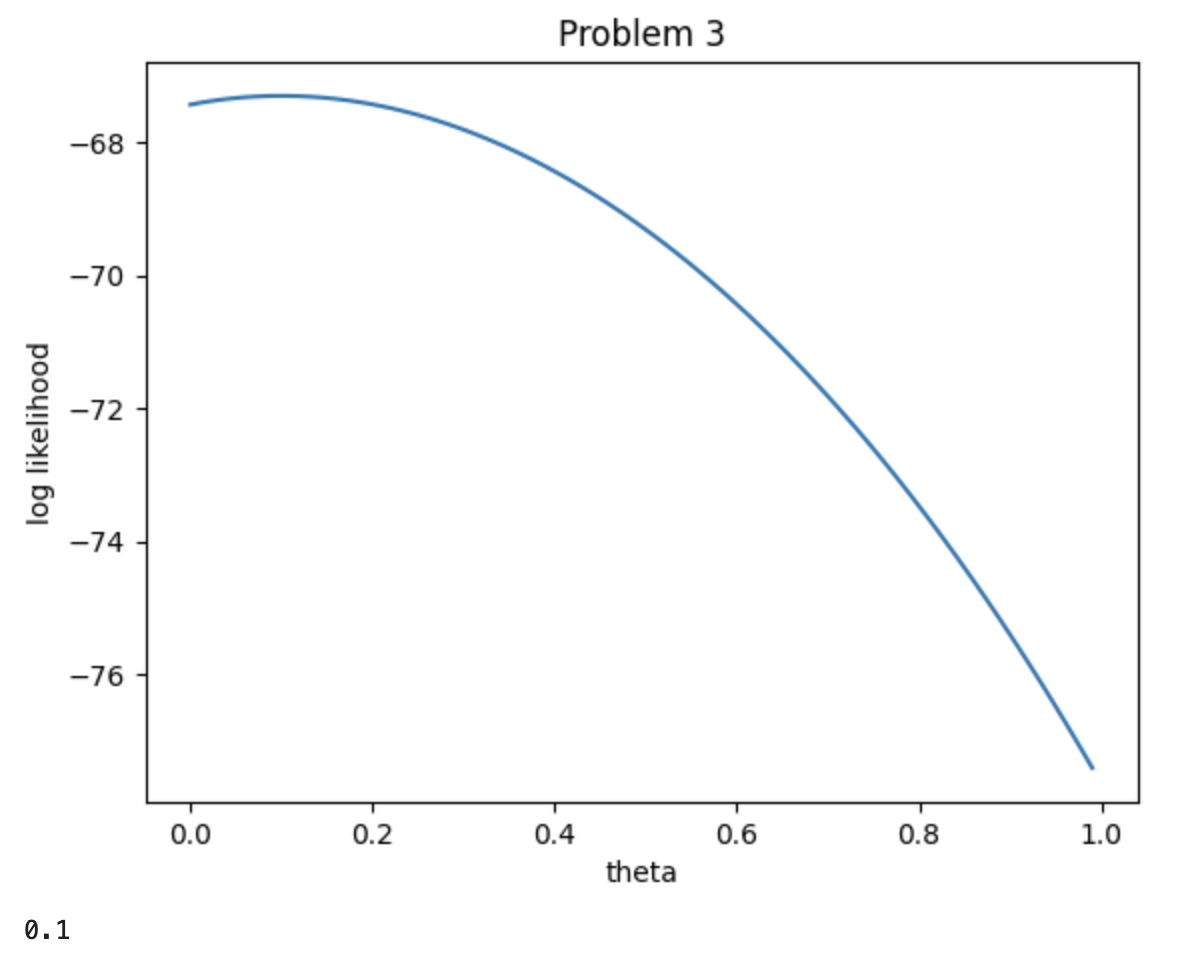
\includegraphics[scale=0.4]{images/p3theta.png}
\end{center}

\newpage
\section{Problem 4}
The set of $x$'s for which $\tilde{f}(x)=3$ is $(6.36336336,\infty)$ \\
Graph and code attached below. Imports omitted.
\begin{minted}[breaklines]{python}
# passing values
mu1, sigma1 = 4.99, 0.31
mu2, sigma2 = 5.93, 0.47
mu3, sigma3 = 6.61, 0.68

# plotting the distributions
x1 = np.linspace(mu1 - 3*sigma1, mu1 + 3*sigma1, 100)
x2 = np.linspace(mu2 - 3*sigma2, mu2 + 3*sigma2, 100)
x3 = np.linspace(mu3 - 3*sigma3, mu3 + 3*sigma3, 100)
plt.plot(x1, stats.norm.pdf(x1, mu1, sigma1), label = "setosa(1)")
plt.plot(x2, stats.norm.pdf(x2, mu2, sigma2), label = "versicolor(2)")
plt.plot(x3, stats.norm.pdf(x3, mu3, sigma3), label = "virginica(3)")
plt.legend()
plt.show()

# find intersections of the distributions
def gaussian(x, mu, sig):
    return 1./(np.sqrt(2.*np.pi)*sig)*np.exp(-np.power((x - mu)/sig, 2.)/2)

x_values = np.linspace(3, 9, 1000)
nd2 = gaussian(x_values, mu2, sigma2)
nd3 = gaussian(x_values, mu3, sigma3)
idx = np.argwhere(np.diff(np.sign(nd2 - nd3))).flatten()
print(x_values[idx]) # prints [4.24324324 6.36336336], which are the two intersections for versicolor and virginica (orange and green)
\end{minted}

\begin{center}
    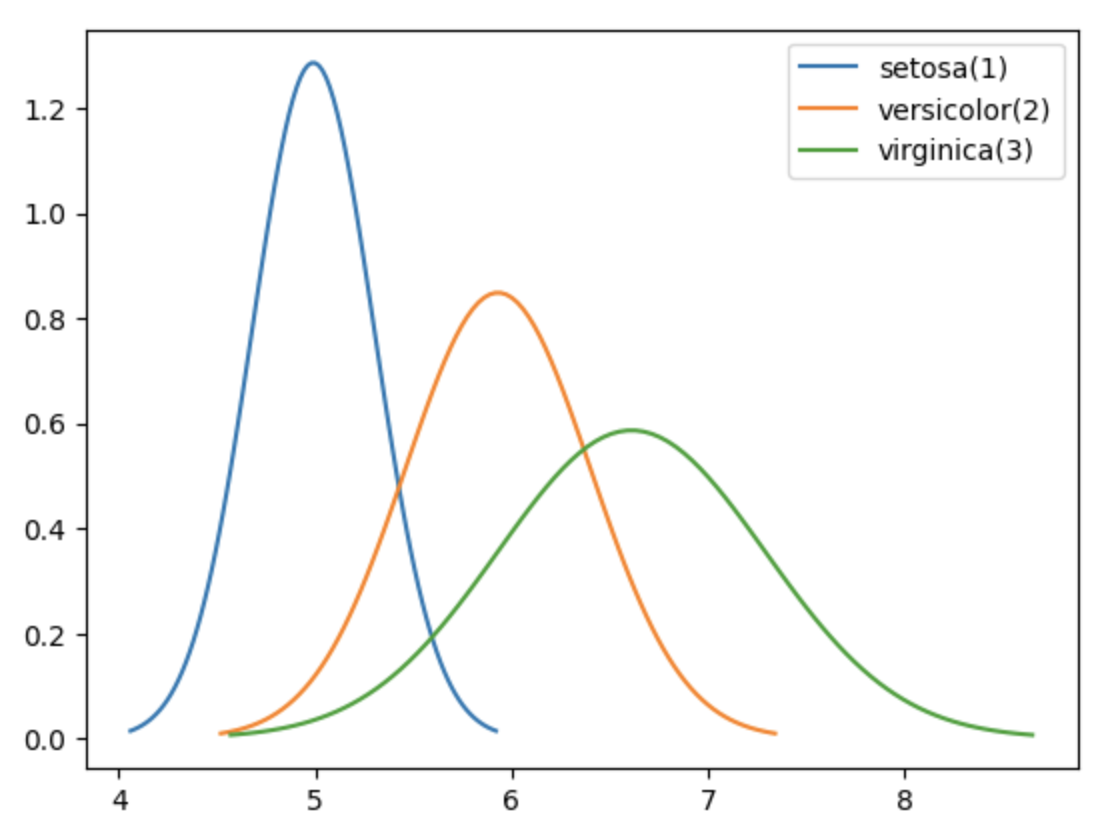
\includegraphics[scale=0.4]{images/p4plot.png}
\end{center}

\newpage
\section{Problem 5}
Consider a test data point $(X,Y)$. For this input to be classified as setosa, the expectation of the loss function when it is classified as setosa should be smaller than the expectation of the loss function when it is classified as versicolor or virginica. In other words, we want $\mathbb{E}_1 (l(X,Y)) < \mathbb{E}_2 (l(X,Y))$ and $\mathbb{E}_1 (l(X,Y)) < \mathbb{E}_3 (l(X,Y))$. \\

The expectation of the loss function can be written as 
\begin{equation}
    \mathbb{E} (l(X,Y)) = \sum \omega P(Y|X)
\end{equation}
where $\omega$ is the respective weight in the loss function. \\

Consider $\mathbb{E}_1 (l(X,Y)) < \mathbb{E}_2 (l(X,Y))$. 
\begin{equation}
    \label{eq:p5}
    \begin{split}
        \mathbb{E}_1 (l(X,Y)) &< \mathbb{E}_2 (l(X,Y)) \\
        2P(Y=2|X) + 2P(Y=3|X) &< P(Y=1|X) \\
        2P(X|Y=2)P(Y=2) + 2P(X|Y=3)P(Y=3) &< P(X|Y=1)P(Y=1) \\
        2P(X|Y=2) + 2P(X|Y=3) &< P(X|Y=1)
    \end{split}
\end{equation}
It turns out that the result acquired from $\mathbb{E}_1 (l(X,Y)) < \mathbb{E}_3 (l(X,Y))$ is exactly the same so we'll just continue with inequality \ref{eq:p5}. \\

Since the distribution of the data  follows the parameters in the normal generative model, we can just plug those values into the inequality. The description of the region where $\tilde{f}=\text{satosa}$ is thus 
\begin{equation}
    \{x \in \mathbb{R} \mid 2*\phi (\frac{x-\mu_2}{\sigma_2}) + 2*\phi (\frac{x-\mu_3}{\sigma_3}) < \phi (\frac{x-\mu_1}{\sigma_1})\}
\end{equation}
% \begin{equation}
%     2* \frac{1}{\sigma_2\sqrt{2\pi}} 
%   \exp\left( -\frac{1}{2}\left(\frac{x-\mu_2}{\sigma_2}\right)^{\!2}\,\right) + 2* \frac{1}{\sigma_3\sqrt{2\pi}} 
%   \exp\left( -\frac{1}{2}\left(\frac{x-\mu_3}{\sigma_3}\right)^{\!2}\,\right) < \frac{1}{\sigma_1\sqrt{2\pi}} 
%   \exp\left( -\frac{1}{2}\left(\frac{x-\mu_1}{\sigma_1}\right)^{\!2}\,\right)
% \end{equation}
where $\mu_1=4.99, \mu_2=5.93, \mu_3=6.61, \sigma_1=0.31, \sigma_2=0.47, \sigma_3=0.68$ \\

Plot the scaled distributions in Python and we get the following plot.
The interval where the inequality is satisfied is (3.63663664 5.27627628). \\ Code attached below. Imports omitted.
\begin{center}
    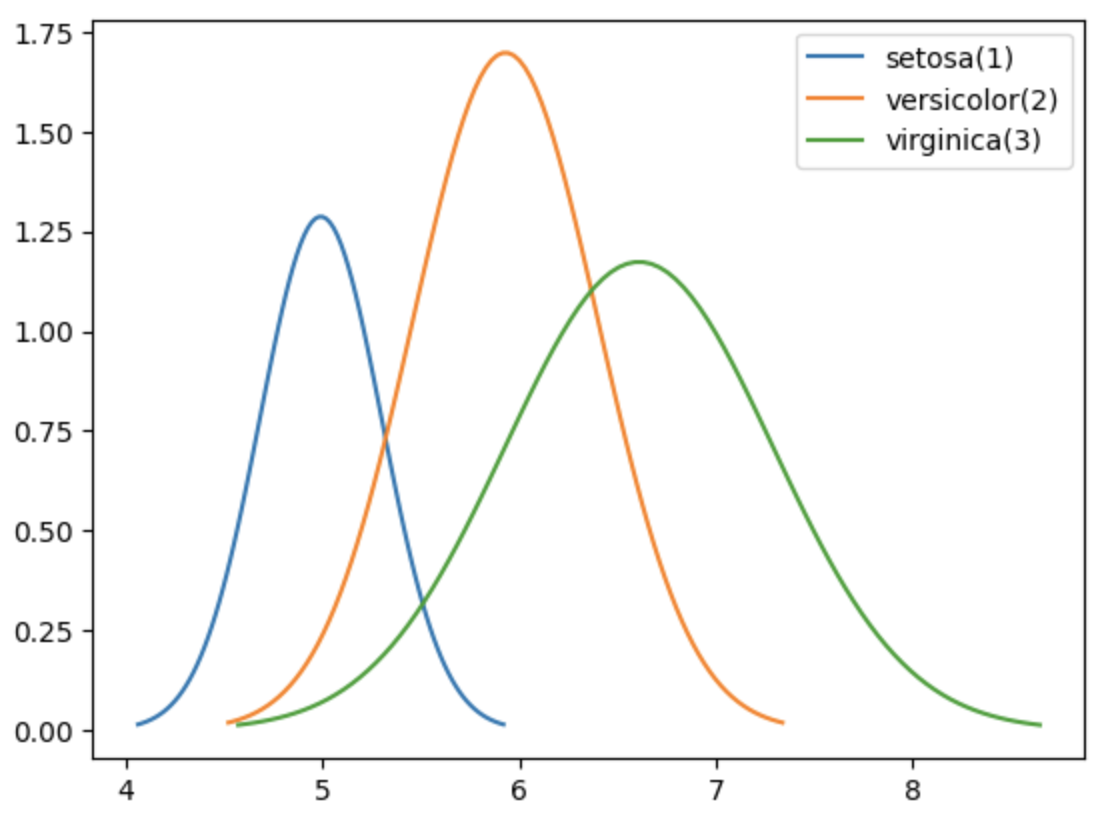
\includegraphics[scale=0.4]{images/p5plot.png}
\end{center}

\begin{minted}[breaklines]{python}
# follow the same distributions
mu1, sigma1 = 4.99, 0.31
mu2, sigma2 = 5.93, 0.47
mu3, sigma3 = 6.61, 0.68

# plot the graphs by scaling the distributions versicolor and virginica by 2
x1 = np.linspace(mu1 - 3*sigma1, mu1 + 3*sigma1, 100)
x2 = np.linspace(mu2 - 3*sigma2, mu2 + 3*sigma2, 100)
x3 = np.linspace(mu3 - 3*sigma3, mu3 + 3*sigma3, 100)
plt.plot(x1, stats.norm.pdf(x1, mu1, sigma1), label = "setosa(1)")
plt.plot(x2, 2*stats.norm.pdf(x2, mu2, sigma2), label = "versicolor(2)")
plt.plot(x3, 2*stats.norm.pdf(x3, mu3, sigma3), label = "virginica(3)")
plt.legend()
plt.show()

# find the intersections to find the solutions to the inequality above
def gaussian(x, mu, sig):
    return 1./(np.sqrt(2.*np.pi)*sig)*np.exp(-np.power((x - mu)/sig, 2.)/2)

x_values = np.linspace(0, 9, 1000)
nd1 = gaussian(x_values, mu1, sigma1)
nd2 = 2*gaussian(x_values, mu2, sigma2)
nd3 = 2*gaussian(x_values, mu3, sigma3)
idx = np.argwhere(np.diff(np.sign(nd1 - (nd2 + nd3)))).flatten()
print(x_values[idx]) # prints [3.63663664 5.27627628]
\end{minted}

\newpage
\section{Problem 6}
To judge whether the training dataset is representative, we need to consider 1. if each data point the dataset is \textbf{independent} of all other data points and 2. if these data points are \textbf{identically distributed}, meaning they follow the same distribution and there is no trend.
\subsection{(a)}
This training dataset is not suitable for the application because it is not representative. \\
Let $(X_i, Y_i)$ denote a data point in the training dataset, where $X_i$ is the feature vector extracted from the articles and $Y_i$ is the number of views received. These $(X_i, Y_i)$ might not be identically distributed, i.e., they might not follow the same distribution. For example, depending on the content of the articles, the time of the publication, and other conditions, the way these articles get "views" might be different.

\subsection{(b)}
This training dataset is not suitable for the application because it is not representative. \\
Let $(X_i, Y_i)$ denote a data point in the training dataset, where $X_i$ is the feature vector extracted from the students and $Y_i$ is whether or not they graduated within four years. These $(X_i, Y_i)$ might not be independent. For example, when a student decides to defer graduation, his friends might also defer graduation...

\subsection{(c)}
This training dataset might be suitable for the application. It is representative. \\
Let $(X_i, Y_i)$ denote a data point in the training dataset, where $X_i$ is the feature vector extracted from the loans and $Y_i$ is whether or not the loan is repaid. Since each loan applicant probably won't know each other, we can consider these $(X_i, Y_i)$ are independent of each other. Also, assume that there is no overall trend to account for in the loan market, these $(X_i, Y_i)$ will pretty much follow the same distribution and are thus identically distributed. Therefore the dataset can be considered representative and constitutes a good training dataset.

\subsection{ps}
Honestly, I feel that all of these training datasets could be used for prediction purposes. It really depends on what kind of results you are looking for, and there's always something you can do to improve the result :)

\end{document}
